\documentclass[10pt,a4paper]{article}
\usepackage[UTF8,fontset = windows]{ctex}
\setCJKmainfont[BoldFont=黑体,ItalicFont=楷体]{华文中宋}
\usepackage{amssymb,amsmath,amsfonts,amsthm,mathrsfs,dsfont,graphicx}
\usepackage{ifthen,indentfirst,enumerate,color,titletoc}
\usepackage{tikz}
\usetikzlibrary{arrows,calc}
\usepackage[bf,small,indentafter,pagestyles]{titlesec}
\usepackage[top=1in, bottom=1in,left=0.8in,right=0.8in]{geometry}
\renewcommand{\baselinestretch}{1.65}
\newtheorem{defi}{定义~}
\newtheorem{eg}{例~}
\newtheorem{ex}{~}
\newtheorem{rem}{注~}
\newtheorem{thm}{定理~}
\newtheorem{coro}{推论~}
\newtheorem{axiom}{公理~}
\newtheorem{prop}{性质~}

\newcommand{\blank}[1]{\underline{\hbox to #1pt{}}}
\newcommand{\bracket}[1]{(\hbox to #1pt{})}

\begin{document}

\begin{center}
    赋能正确率介于$0.75$至$0.85$的题目
\end{center}

{\tiny 1,7,0.814}  抛掷一枚均匀的骰子(刻有1、2、3、4、5、6)三次, 得到的数字依次记作$a$、$b$、$c$, 则$a+b\mathrm{i}$($\mathrm{i}$为虚数单位)是方程$x^2-2x+c=0$的根的概率是\blank{50}.

{\tiny 1,8,0.814}  设常数$a>0$, $(x+\dfrac{a}{\sqrt{x}})^9$展开式中$x^6$的系数为$4$, 则$\displaystyle\lim_{n\to \infty}(a+a^2+\cdots+a^n)=$\blank{50}.

{\tiny 2,2,0.814} 已知抛物线$C$的顶点在平面直角坐标系原点, 焦点在$x$轴上, 若$C$经过点$M(1,3)$, 则其焦点到准线的距离为\blank{50}.

{\tiny 2,8,0.791} 如图, 在$\triangle ABC$中, 若$AB=AC=3$, $\cos \angle BAC=\dfrac{1}{2}$, $\overrightarrow{DC}=2\overrightarrow{BD}$, 则$\overrightarrow{AD}\cdot \overrightarrow{BC}=$\blank{50}.
\begin{center}
    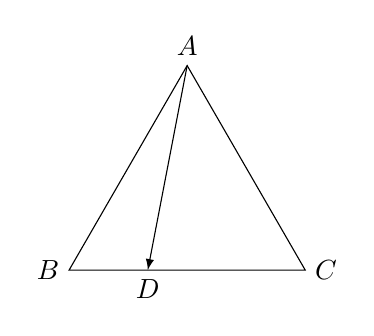
\begin{tikzpicture}[>=latex]
        \draw (0,0) node [left] {$B$} -- (3,0) node [right] {$C$} -- (1.5,{1.5*sqrt(3)}) node [above] {$A$} coordinate (A) -- cycle;
        \draw [->] (A) -- (1,0) node [below] {$D$};
    \end{tikzpicture}
\end{center}

{\tiny 3,6,0.791} 甲、乙两人从$5$门不同的选修课中各选修$2$门, 则甲、乙所选的课程中恰有$1$门相同的选法有\blank{50}种.

{\tiny 7,6,0.818} 里约奥运会游泳小组赛采用抽签方法决定运动员比赛的泳道, 在由$2$名中国运动员和$6$名外国运动员组成的小组中, $2$名中国运动员恰好抽在相邻泳道的概率为\blank{50}.

{\tiny 8,6,0.795} 已知$f(x)=\sin\dfrac\pi 3x$, $A=\{1,2,3,4,5,6,7,8\}$, 现从集合$A$中任取两个不同元素$s$、$t$, 则使得$f(s)\cdot f(t)=0$发生的概率是\blank{50}.

{\tiny 8,9,0.773} 将边长为$10$的正三角形$ABC$, 按``斜二测''画法在水平放置的平面上画出为$\triangle A'B'C'$, 则$\triangle A'B'C'$中最短边的边长为\blank{50}(精确到0.01).

{\tiny 10,2,0.780} 三阶行列式$\begin{vmatrix}   3 & -5 & 1 \\   2 & 3 & -6 \\   -7 & 2 & 4 \\ \end{vmatrix}$中元素$-5$的代数余子式的值为\blank{50}.

{\tiny 12,5,0.841} 用半径$1$米的半圆形薄铁皮制作圆锥型无盖容器, 其容积为\blank{50}立方米.

{\tiny 12,8,0.773} 在无穷等比数列$\{a_n\}$中, $\displaystyle\lim_{n\to\infty}(a_1+a_2+\cdots+a_n)=\dfrac12$, 则$a_1$的取值范围是\blank{50}.

{\tiny 12,9,0.841} 某班班会准备从含甲、乙的$6$名学生中选取$4$人发言, 要求甲、乙两人至少有一人参加, 那么不同的发言顺序有\blank{50}种.

{\tiny 16,10,0.837} 设焦点为$F_1$、$F_2$的椭圆$\dfrac{x^2}{a^2}+\dfrac{y^2}3=1 \ (a>0)$上的一点$P$也在抛物线$y^2=\dfrac94x$上, 抛物线焦点为$F_3$, 若$|PF_3|=\dfrac{25}{16}$, 则$\triangle PF_1F_2$的面积为\blank{50}.

% 赋能17


{\tiny 19,9,0.814} 数列$\{a_n\}$的通项公式是$a_n=2n-1\ (n\in \mathbf{N}^*)$, 数列$\{b_n\}$的通项公式是$b_n=3n \ (n\in \mathbf{N}^*)$, 令集合$A=\{a_1,a_2,\cdots,a_n,\cdots\}$, $B=\{b_1,b_2,\cdots,b_n,\cdots\}$, $n\in \mathbf{N}^*$. 将集合$A\cup B$中的所有元素按从小到大的顺序排列, 构成的数列记为$\{c_n\}$. 则数列$\{c_n\}$的前$28$项的和$S_{28}=$\blank{50}.

{\tiny 20,10,0.837}  已知函数$f(x)=\begin{cases} (5-a)x+1, & x<1, \\ a^x, & x\ge 1\end{cases} \ (a>0,a\ne 1)$是实数集$\mathbf{R}$上的增函数, 则实数$a$的取值范围为\blank{50}.

% 赋能21


{\tiny 21,1,0.818} 集合$P=\{x|0 \le x<3, x\in \mathbf{Z}\}$, $M=\{x|x^2 \le 9\}$, 则$P\cap M=$\blank{50}.

{\tiny 22,5,0.810} 不等式$\dfrac1{|x-1|}\ge 1 $的解集为\blank{50}.

{\tiny 22,10,0.810} 设$a_1,a_2,a_3,a_4$是$1,2,3,4$的一个排列, 若至少有一个$i\ (i=1,2,3,4)$使得$a_i=i$成立, 则满足此条件的不同排列的个数为\blank{50}.

% 赋能23


{\tiny 23,9,0.795} 在$\triangle ABC$中, $\angle A=90^\circ $, $\triangle ABC$的面积为$1$. 若$\overrightarrow{BM}=\overrightarrow{MC}$, $\overrightarrow{BN}=4 \overrightarrow{NC}$, 则$\overrightarrow{AM}\cdot \overrightarrow{AN}$的最小值为\blank{50}.

{\tiny 26,7,0.837} 数列$\{a_n\}$的前$n$项和为$S_n$, 若点$(n,S_n) \ (n\in \mathbf{N}^*)$在函数$y=\log_2 (x+1)$的反函数的图像上, 则$a_n$=\blank{50}.

{\tiny 26,9,0.814} 抛物线$y^2=-8x$的焦点与双曲线$\dfrac{x^2}{a^2}-y^2=1$的左焦点重合, 则这条双曲线的两条渐近线的夹角为\blank{50}.

{\tiny 27,10,0.814} 已知数列$\{a_n\}$的前$n$项和为$S_n$, 且$a_1=1$, $2S_n=a_na_{n+1}$($n\in \mathbf{N}^*$), 若$b_n=(-1)^n\dfrac{2n+1}{{a_n}{a_{n+1}}}$, 则数列$\{b_n\}$的前$n$项和$T_n=$\blank{50}.

%赋能28


{\tiny 28,9,0.837} 已知函数$f(x)=\begin{cases} \log_2 x, & 0<x<2, \\ (\dfrac23)^x+\dfrac59, & x\ge 2. \end{cases}$ 若函数$g(x)=f(x)-k$有两个不同的零点, 则实数$k$的取值范围是\blank{50}.

{\tiny 29,10,0.837} 若三棱锥$S-ABC$的所有的顶点都在球$O$的球面上, $SA\perp$平面$ABC$, $SA=AB=2$, $AC=4$, $\angle BAC=\dfrac{\pi}3$, 则球$O$的表面积为\blank{50}.

% 赋能30


{\tiny 30,8,0.837} 在约束条件$|x+1|+|y-2|\le 3$下, 目标函数$z=x+2y$的最大值为\blank{50}.

{\tiny 32,10,0.767} 三条侧棱两两垂直的正三棱锥, 其俯视图如图所示, 主视图的边界是底边长为$2$的等腰三角形, 则主视图的面积等于\blank{50}.
\begin{center}
    \begin{tikzpicture}[scale = 1.5, >=latex]
        \draw (0,0) -- (2,0) -- (1,{sqrt(3)}) coordinate (T) -- cycle;
        \draw (0,0) -- (1,{sqrt(3)/3}) -- (2,0) (1,{sqrt(3)/3}) -- (1,{sqrt(3)});
        \draw (0,-0.1) -- (0,-0.3) (2,-0.1) -- (2,-0.3);
        \draw (1,-0.2) node {$2$};
        \draw [->] (0.8,-0.2) -- (0,-0.2);
        \draw [->] (1.2,-0.2) -- (2,-0.2);
        \draw (1,-0.5) node {俯视图};
        \draw (2,0) ++ (30:0.1) --++ (30:0.2) (T) ++ (30:0.1) --++ (30:0.2);
        \draw [->] ($(2,0)!0.4!(T)$) ++ (30:0.2) --+ (-60:0.8);
        \draw [->] ($(2,0)!0.6!(T)$) ++ (30:0.2) --+ (120:0.8);
        \draw ($(2,0)!0.5!(T)$) ++ (30:0.2) node {$2$};
        \draw (0,0) ++ (150:0.1) --++ (150:0.2) (T) ++ (150:0.1) --++ (150:0.2);
        \draw [->] ($(0,0)!0.4!(T)$) ++ (150:0.2) --+ (240:0.8);
        \draw [->] ($(0,0)!0.6!(T)$) ++ (150:0.2) --+ (60:0.8);
        \draw ($(0,0)!0.5!(T)$) ++ (150:0.2) node {$2$};
    \end{tikzpicture}
\end{center}

% 赋能33


{\tiny 33,10,0.810} 若将函数$f(x)=|\sin(\omega x-\dfrac{\pi}8)| \ (\omega >0)$的图像向左平移$\dfrac{\pi}{12}$个单位后, 所得图像对应的函数为偶函数, 则$\omega$的最小值是\blank{50}.

% 赋能34


{\tiny 34,8,0.791} 已知正四棱锥$P-ABCD$的棱长都相等, 侧棱$PB$、$PD$的中点分别为$M$、$N$, 则截面$AMN$与底面$ABCD$所成的二面角的余弦值是\blank{50}.

{\tiny 34,10,0.837} 若适合不等式$|x^2-4x+k|+|x-3|\le 5$的$x$的最大值为$3$, 则实数$k$的值为\blank{50}.

% 赋能35


{\tiny 35,10,0.791} 已知定义在$\mathbf{R}$上的函数$f(x)$满足: \textcircled{1} $f(x)+f(2-x)=0$; \textcircled{2} $f(x)-f(-2-x)=0$; \textcircled{3} 在$[-1,1]$上的表达式为$f(x)=\begin{cases} \sqrt{1-x^2}, & x\in [-1,0], \\ 1-x, & x\in (0,1] \end{cases}$, 则函数$f(x)$与函数$g(x)=\begin{cases} 2^x, & x\le 0, \\ \log_{\frac12} x,& x>0 \end{cases}$的图像在区间$[-3,3]$上的交点的个数为\blank{50}.

% 赋能36


{\tiny 36,5,0.786} 若圆锥的侧面积是底面积的$2$倍, 则其母线与轴所成角的大小是\blank{50}.

{\tiny 37,5,0.791} 若圆柱的侧面展开图是边长为$4\text{cm}$的正方形, 则圆柱的体积为\blank{50}$\text{cm}^3$(结果精确到$0.1\text{cm}^3$).

{\tiny 41,8,0.837} 无穷等比数列$\{a_n\}$的通项公式$a_n=(\sin x)^n$, 前$n$项的和为$S_n$, 若$\displaystyle\lim_{n\to\infty}S_n=1$, $x\in (0,\pi)$, 则$x=$\blank{50}.

{\tiny 41,9,0.767} 给出下列函数: \textcircled{1} $y=x+\dfrac1x$; \textcircled{2} $y={x^2}+x$; \textcircled{3} $y={2^{|x|}}$; \textcircled{4} $y={x^{\dfrac23}}$; \textcircled{5} $y=\tan x$; \textcircled{6} $y=\sin(\arccos x)$; \textcircled{7} $y=\lg(x+\sqrt{{x^2}+4})-\lg 2$. 从这$7$个函数中任取两个函数, 则其中一个是奇函数另一个是偶函数的概率是\blank{50}.

{\tiny 42,10,0.837} 已知直线$l_1:mx-y=0$, $l_2:x+my-m-2=0$. 当$m$在实数范围内变化时, $l_1$与$l_2$的交点$P$恒在一个定圆上, 则定圆方程是\blank{50}.

% 赋能43


{\tiny 43,6,0.837} 从集合$\{-1,1,2,3\}$随机取一个为$m$, 从集合$\{-2,-1,1,2\}$随机取一个为$n$, 则方程$\dfrac{x^2}m+\dfrac{y^2}n=1$表示双曲线的概率为\blank{50}.

{\tiny 43,10,0.791} 椭圆的长轴长等于$m$, 短轴长等于$n$, 则此椭圆的内接矩形的面积的最大值为\blank{50}.

% 赋能44


{\tiny 44,7,0.791} 已知函数$f(x)=\begin{vmatrix}
2\sin x & -\cos 2x  \\ 1  & \cos x  \end{vmatrix}$, 则函数$f(x)$的单调递增区间是\blank{50}.

{\tiny 45,9,0.837} $(1+2x)^n$的二项展开式中, 含$x^3$项的系数等于含$x$项的系数的$8$倍, 则正整数$n=$\blank{50}.

{\tiny 46,5,0.767} 如图的三个直角三角形是一个体积为$20\text{cm}^3$的几何体的三视图, 则$h=$\blank{50}.
\begin{center}
    \begin{tikzpicture}[>=latex]
        \draw (0,0) -- (2.5,0) -- (0,2) -- cycle;
        \draw (0,-0.1) -- (0,-0.3) (2.5,-0.1) -- (2.5,-0.3);
        \draw (1.25,-0.2) node {$5$};
        \draw [->] (1.05,-0.2) -- (0,-0.2);
        \draw [->] (1.45,-0.2) -- (2.5,-0.2);
        \draw (1.25,-0.5) node {主视图};
        \draw (-0.1,0) -- (-0.3,0) (-0.1,2) -- (-0.3,2);
        \draw (-0.2,1) node {$h$};
        \draw [->] (-0.2,0.8) -- (-0.2,0);
        \draw [->] (-0.2,1.2) -- (-0.2,2);
        \draw (3.5,0) -- (6.5,0) -- (3.5,2) -- cycle;
        \draw (3.5,-0.1) -- (3.5,-0.3) (6.5,-0.1) -- (6.5,-0.3);
        \draw (5,-0.2) node {$6$};
        \draw [->] (4.8,-0.2) -- (3.5,-0.2);
        \draw [->] (5.2,-0.2) -- (6.5,-0.2);
        \draw (5,-0.5) node {左视图};
        \draw (0,-1) -- (2.5,-1) -- (0,-4) -- cycle;
        \draw (1.25,-4.5) node {俯视图};
    \end{tikzpicture}
\end{center}

{\tiny 48,9,0.814} 已知抛物线型拱桥的顶点距水面$2$米时, 量得水面宽为$8$米. 当水面下降$1$米后, 水面的宽为\blank{50}米.

{\tiny 49,9,0.814} 设函数$f(x)=\log_m x$($m>0$且$m\ne 1$), 若$m$是等比数列$\{a_n\}$($n\in \mathbf{N}^*$)的公比, 且$f(a_2a_4a_6\cdots a_{2018})=7$, 则$f(a_1^2)+f(a_2^2)+f(a_3^2)+\cdots+f(a_{2018}^2)$的值为\blank{50}.

{\tiny 50,9,0.791} 已知$f(x)$是定义在$[-2,2]$上的奇函数, 当$x\in (0,2]$时,$f(x)=2^x-1$, 函数$g(x)=x^2-2x+m$. 如果对于任意的$x_1\in [-2,2]$, 总存在$x_2\in [-2,2]$, 使得$f(x_1)\le g(x_2)$, 则实数$m$的取值范围是\blank{50}.

{\tiny 51,9,0.791} 若$\sin(x-y)\cos x-\cos(x-y)\sin x=\dfrac35$, 则$\tan 2y$的值为\blank{50}.

{\tiny 54,7,0.837} 设定义在$\mathbf{R}$上的奇函数$y=f(x)$, 当$x>0$时, $f(x)=2^x-4$, 则不等式$f(x)\le 0$的解集是\blank{50}.

{\tiny 55,10,0.767} 现有$5$位教师要带$3$个班级外出参加志愿者服务, 要求每个班级至多两位老师带队, 且教师甲、乙不能单独带队, 则不同的带队方案有\blank{50}(用数字作答).

% 赋能56


{\tiny 56,7,0.837} 函数$y=\sqrt{x^2+2}+\dfrac1{\sqrt{x^2+2}}$的最小值为\blank{50}.

{\tiny 56,8,0.837} 试写出$(x-\dfrac1x)^7$展开式中系数最大的项\blank{50}.

{\tiny 57,2,0.814} 已知集合$A=\{x||x-2|<a\}$, $B=\{x|x^2-2x-3<0\}$, 若$B\subseteq A$, 则实数$a$的取值范围是\blank{50}.

{\tiny 57,6,0.767} 已知$F_1,F_2$是椭圆$C:\dfrac{x^2}{a^2}+\dfrac{y^2}{b^2}=1\ (a>b>0)$的两个焦点, $P$为椭圆上一点, 且$\overrightarrow{PF_1}\perp \overrightarrow{PF_2}$, 若$\triangle PF_1F_2$的面积为$9$, 则$b=$\blank{50}.

{\tiny 57,8,0.791} 设等差数列$\{a_n\}$的公差为$d$, 若$a_1,a_2,a_3,a_4,a_5,a_6,a_7$的方差为$1$, 则$d$=\blank{50}.

{\tiny 58,1,0.791} 设集合$M=\{x|x^2=x\}$, $N=\{x|\log_2 x\le 0\}$, 则$M\cup N=$\blank{50}.

{\tiny 58,7,0.837} 若行列式$\begin{vmatrix}   1 & 2 & 4 \\   \cos (\pi +x) & 2 & 0 \\   -1 & 1 & 6 \end{vmatrix}$中的元素$4$的代数余子式的值等于$\dfrac32$, 则实数$x$的取值集合为\blank{50}.





\end{document}